\chapter[Metodologia]{Metodologia}

A metodologia utilizada será a pesquisa exploratória utilizando da revisão sistemática para encontrar a resposta à seguinte pergunta: “ Uma vez definido os indicadores das métricas, como criar uma interface de visualização da informação para um orgão público federal? ”. O uso da pesquisa exploratória se deu por conta da baixa produção de artigos na área. A revisão sistemática é uma técnica criada na área da medicina que se difundiu para outras áreas de conhecimento por causa da produtividade que se ganha ao se deparar com um conjunto de artigos que não se sabe quais que se adequam ao conteúdo do autor. A revisão sistemática se dará em três etapas consecutivas: planejamento, execução e analise.


\begin{table}[http]
	\centering
	\caption{Cronograma TCC 1}
	\label{tab:cronograma}
	\begin{tabular}{ccccc}
		\hline
		\multicolumn{1}{|c|}{\textbf{Cronograma}}             & \multicolumn{1}{c|}{\textbf{Agosto}} & \multicolumn{1}{c|}{\textbf{Setembro}} & \multicolumn{1}{c|}{\textbf{Outubro}} & \multicolumn{1}{c|}{\textbf{Novembro}} \\ \hline
		\multicolumn{1}{|c|}{Realizar Pesquisa Bibliográfica} & \multicolumn{1}{c|}{X}              & \multicolumn{1}{c|}{X}              & \multicolumn{1}{c|}{X}             & \multicolumn{1}{c|}{X}              \\ \hline
		\multicolumn{1}{|c|}{Estudar o orgão}             & \multicolumn{1}{c|}{}               & \multicolumn{1}{c|}{X}              & \multicolumn{1}{c|}{X}             & \multicolumn{1}{c|}{}               \\ \hline
		\multicolumn{1}{|c|}{Propor Versão Inicial do dashboard}                & \multicolumn{1}{c|}{}               & \multicolumn{1}{c|}{}               & \multicolumn{1}{c|}{X}             & \multicolumn{1}{c|}{X}              \\ \hline
		\multicolumn{1}{l}{}                                  & \multicolumn{1}{l}{}                & \multicolumn{1}{l}{}                & \multicolumn{1}{l}{}               & \multicolumn{1}{l}{}                \\
		\multicolumn{1}{l}{}                                  & \multicolumn{1}{l}{}                & \multicolumn{1}{l}{}                & \multicolumn{1}{l}{}               & \multicolumn{1}{l}{}                \\
		\multicolumn{1}{l}{}                                  & \multicolumn{1}{l}{}                & \multicolumn{1}{l}{}                & \multicolumn{1}{l}{}               & \multicolumn{1}{l}{}               
	\end{tabular}
\end{table}



\graphicspath{{figuras/}}
\begin{figure}[!htb]
\centering
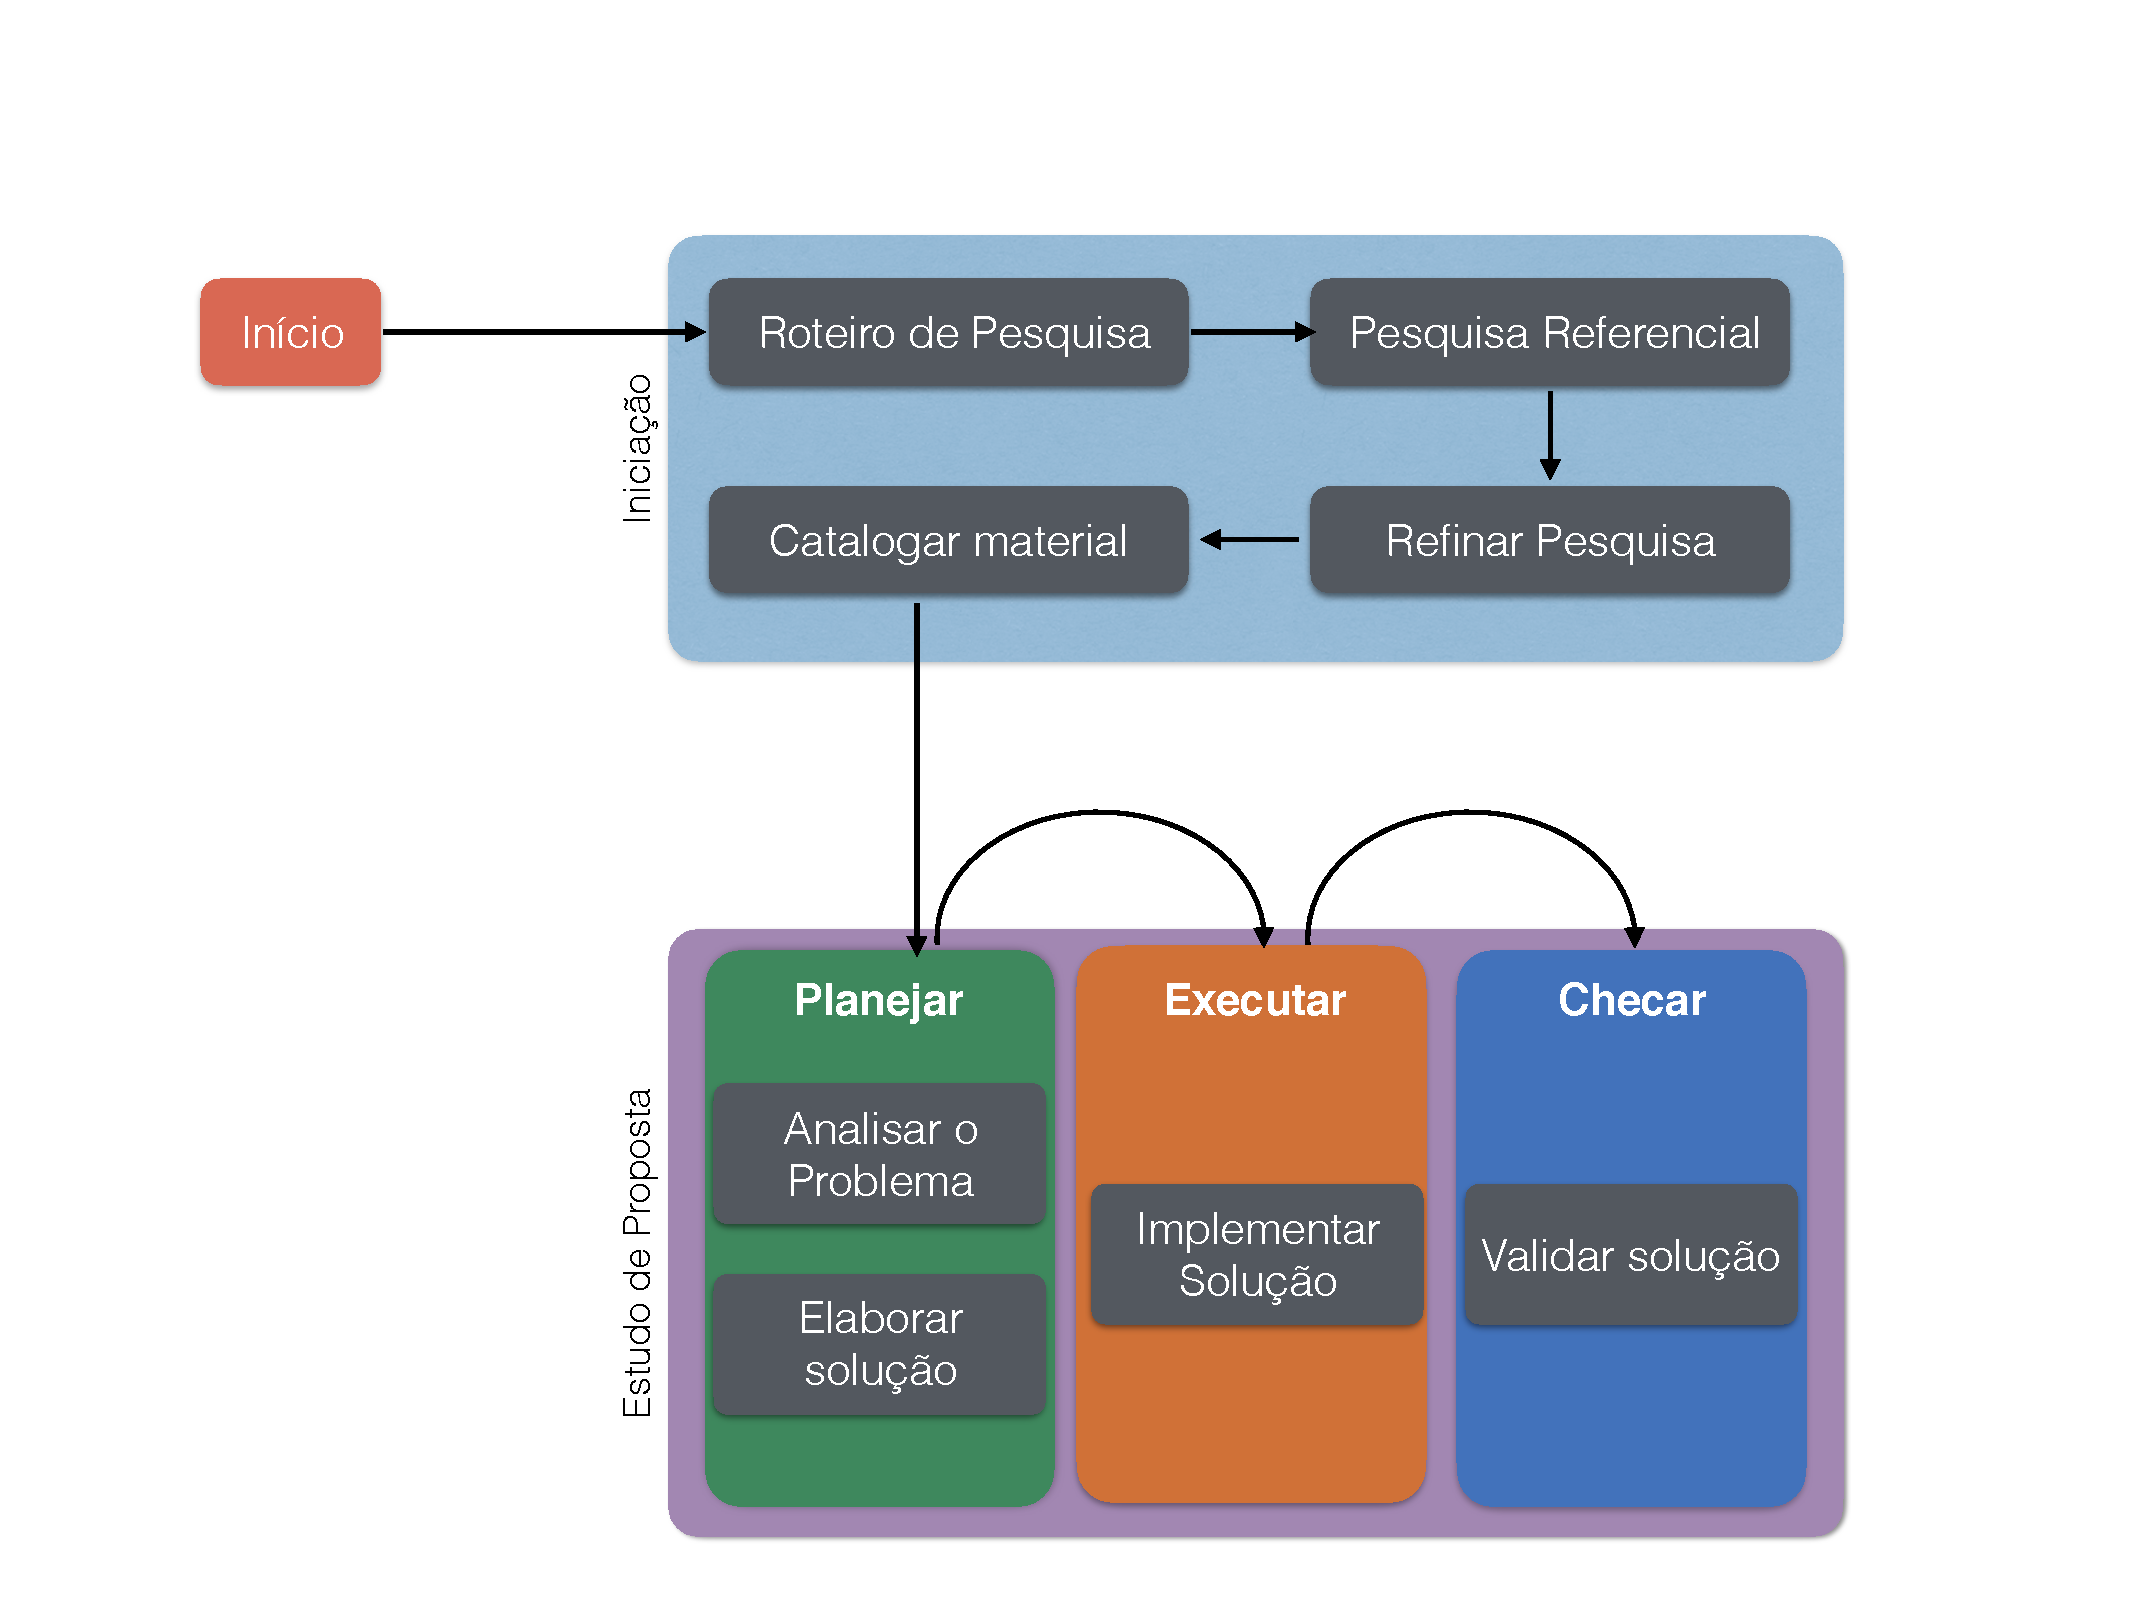
\includegraphics[scale=0.5]{TCCMetodologia}
\caption{Plano de Pesquisa}
\label{Rotulo}
\end{figure}
